%===================================================================================================
%  Chapter : 運動学
%  説明    : 物体の運動の表現方法について,記述する.
%===================================================================================================
%   %======================================================================
%   % Section
%   %======================================================================
    \section{「物体の運動」の表現方法}
    \begin{mycomment}
        物理学,特に力学の主な目的は,物体の運動軌道を(数学的に)推測する
        ことにある.これから学習する力学は,スペースシャトルを地球から宇宙へ飛ばす
        際に実際に使われる理論でもある.また,アメリカの人類初の月面着陸(1969)を実現
        するにも,この力学理論が使われている
            \footnote{
                もちろん,力学だけではない.スペースシャトルや宇宙服などに使われる装置
                を作る際に用いられる理論は,
                電磁気学,物性理論,電子回路論,材料工学など様々なものが使われている.
                しかし,スペースシャトルの打ち上げ方向を決めるのには,力学理論以外には,
                何も使用していない.摩擦や,宇宙での人間の行動を考えずに,単に宇宙に飛び出して
                月に行くことだけを考えれば,250年前にニュートンが創り上げた力学理論さえあれば
                よいのである.
            }.

       物体の運動を表すには,どのような概念があるとよいのかを,この節で説明していこう.
    \end{mycomment}
%       %======================================================================
%       %  SubSection
%       %======================================================================
        \subsection{位置}
        物理学の,ここでは特にニュートン力学の重要な目的の1つに,\textbf{物体の
        運動を記述する} ことがある.記述の仕方はどのようであってもよいが,最もよ
        く表現できる道具として,数式が有力である.実際に,物理学では物体の運動を
        数式を用いて表現している.数式で表現すれば,曖昧さ無しに,誰にでも全く同
        一のイメージを与えることができる.

        物体の運動は数式を用いて行うことはわかった.では,実際に数式で表現するに
        はどうすればよいだろうか.物体の運動を記述したいのであるから,まず“物体
        がどこに存在するかを示す指標”が必要になる.この指標のことを,\textbf{位置} と
        いう.物体はいつも同じ場所に存在しているとは限らない.時々刻々と,その位
        置を変化させている物体のほうが一般的である
            \footnote{
                少なくとも,地球上の物体(私たちの体を含めて)は,時々刻々とその
                位置を変化させている.なぜなら,地球は太陽に対して公転しているの
                であるから,地球の外側(宇宙)から見れば,地球上の物体はすべて動
                いているのである.
            }.

%       %======================================================================
%       %  SubSection
%       %======================================================================
        \subsection{速度}
        物体の位置が記述できれば,それだけで物体の運動を記述でるだろうか.否,
        明らかに不可能である.物体が“どのように”運動しているかということも,
        記述すべきだ.つまり,物体の \textbf{速度} も知っておかないと
        いけない情報の1つである.速度とは,単位時間あたりに,物体がどの程度
        移動したかを示す指標である.

%       %======================================================================
%       %  SubSection
%       %======================================================================
        \subsection{加速度}
        さらに言うと,物体の速度は常に一定であることは珍しく,速度も位置と同様に,
        時々刻々と変化している方が一般的である.この速度の時間変化のことを,
        \textbf{加速度} という.

            \begin{memo}{加加速度,躍度,jerk}
                「速度」,「加速度」とくれば,「加加速度」というものも
                考えられるのではないか.実際,その通りで,
                加加速度という概念は存在している.これは,「躍度(やくど)」と
                も言われる.英単語では,jerkがそれに相当する.
                加速度が急激に変化すると,機械におおきな負担がかかること
                になる.この負担を数値で示すのが,躍度である.

                ニュートンの運動の第2法則(運動方程式)で,加速度と力は比例関係にある
                ことが分かっているので,躍度とは力の時間変化であると言い換えることも
                できる.

                なお,ニュートン力学を学ぶにあたり,躍度という概念は
                使うことはない.
            \end{memo}


%       %======================================================================
%       %  SubSection
%       %======================================================================
        \subsection{運動軌道}
        物体が,ある位置で突然と消えてしまい,次の瞬間に全く別の場所から突然現れ
        ることはない
            \footnote{
                実は,このことは後で考える \textbf{エネルギー保存の法則} に関連
                したことである.
            }.
        つまり,言い方を変えれば,時間的に位置が変化する物体について,その位置を
        時刻ごとに記録していけば,物体の \textbf{軌道} を得られるということであ
        る.実はこの物体の軌道こそが,ニュートン力学で興味ある事なのである.物体
        の運動の記述をするということは,物体の運動軌道を記述するということなので
        ある.

        では,物体の軌道を記述するには,どうしたらよいだろうか.観測できるのは,
        物体の持つ今この瞬間の性質であり,一瞬にして運動軌道を得ることはできない.
        もちろん,時間をかけて観測すればその軌道は明らかになるが,この観測でわかる
        のは,観測の対象としている物体の軌道のみであり,一般の物体についてのもので
        はない.知りたいのは,「現在の物体のもつ運動状況」から物体の軌道を推測する
        方法である.

%       %======================================================================
%       %  SubSection
%       %======================================================================
        \subsection{「運動の軌道」の表現に必要な情報}
        物体の運動を記述するということは,物体の動く道筋である
        運動の軌跡を記述するということである.そして,物体の運動の軌跡を記述する
        には,物体の位置・速度・加速度の3つが必要である.さらに,物体の位置や速
        度は時間的に変化するものなので,当然,「時刻」も必要である.この4つの要
        素を基に,数式を用いた推論を行うことで,物体の軌道を表現できる.

        ここに挙げた4つの概念,つまり,時刻・位置・速度・加速度は,数式で扱う以上,
        何らかの文字で表す必要がある.そこで,これら4つに次のように文字を割当て
        ることにする.
        \begin{myshadebox}{運動の軌跡の表現に必要なもの}
            物体の運動を数式で表現するには,次の4つの要素が必要である.
            \begin{enumerate}
                \item 時刻:$t$
                \item 位置:$\br$
                \item 速度:$\bv$
                \item 加速度:$\ba$
            \end{enumerate}
        \end{myshadebox}

        なぜ時刻を表す $t$ は普通の太さなのに,他の3つの位置 $\br$,速度 $\bv$,
        加速度 $\ba$ は太文字で表現されるかという,疑問があることと思う.これに
        ついては,この後に説明する.ここでは,このような文字が割当てられている
        ということを,知ることができれば十分である.

        ちなみに,このようなアルファベット($t$,$\br$,$\bv$,$\ba$)を割
        当てる強い理由はない.大切なのは,文字に意味を割当てるということであり,
        文字が何を意味するかではない.どのような文字を割当てても,全く同じよう
        に議論できることは明白である.ここでは,単に慣習に従って
            \footnote{
                私は単に多くの教科書で採用されている記号を流用しているに過ぎない.
                偉そうなことを書いたが,教科書でなぜこのように文字を割当ててい
                るのかは分かっていない.
            },
        時刻 $t$/位置 $\br$/速度 $\bv$/加速度 $\ba$ と割当てただけである.
        英単語を見てみると,
        時間はtime,点(位置)はrespect,速度はvelocity,加速度はacceleration
        である.その頭文字をとっているのかもしれない.

%   %==========================================================================
%   %  Section
%   %==========================================================================
    \section{位置の記述方法}
        \begin{mycomment}
            物体の存在する位置(場所)を表現することを考えてみよう.
            例えば,物体が「ここにある」とか「あそこにある」
            といっても,見る人によって見える方向は違ってくる.
            例えば,二人の人間の真中に静止している
            ボールがあるとして,そのボールは一方の人から見れば
            「右側」にあるというだろうし,
            もう一人は「左側」にあるというだろう.この場合,
            ボールが静止しているのにもかかわらず,
            二人のボールの位置に関する主張は異なっている.
            これではどうにもこうにも話が進まない.
            ここでは,この問題を解決することを考える.
        \end{mycomment}


%       %======================================================================
%       %  SubSection
%       %======================================================================
        \subsection{1次元(直線)上の位置}
                まず,最も簡単な直線上の位置を表すことを考えてみよう.
                その方法とは,
                直線の各点に数字を貼り付けて,その数字によって位置を表すというものである.
                図\ref{fig:ichi1}参照.
                このように直線上で表される位置を,\textbf{1次元} という.
                \begin{figure}[hbt]
                    \begin{center}
                        \includegraphicsdefault{ichi_1jigen.pdf}
                        \caption{1次元(直線上)での位置}
                        \label{fig:ichi1}
                    \end{center}
                \end{figure}

                位置を指定したいときは,まず,「基準」とする位置を決める必要がある.
                この基準の位置は直線上であればどこでもよいが,一度基準の位置を決めたら絶対にこの基準を
                変更してはいけない.基準はOと表記される.
                この基準から左右の直線に,数字を貼り付けていく.
                そして,直線上の物体の位置をその実数で表すのである.ここで大切なことは,
                \textbf{位置と実数が1対1に対応している} ことである
                        \footnote{
                        “1対1に対応している”ということは,『
                        位置を1つ指定したならば,それに対応する実数が1つだけに決まり,
                        逆に数字を1つ指定したならば,それに対応する位置が1つだけに定まる』ということである.
                        }.
                図\ref{fig:ichi1}で,
                点Bの位置を示すときには,$-2$といえばよい.同様に,点Aを示すには$-6$を,点Dを
                示すには$3.9$をいえばよい.つまり,「点の位置は$-2$である」とか,「点の位置は3.9である」
                とかといって,位置を表現するのである.数式的に書けば,例えば点Bの位置が$-2$であるならば
                    \begin{equation*}
                        \mbox{点{\rm B}の位置} = -2
                    \end{equation*}
                のように書けるだろう.“点の位置”という日本語ではこれから式を扱っていく上で
                不都合があるから,これを記号で表現しようと思う.すなわち
                位置を表す記号を導入し,これを $r$ と書くことにするということだ.
                すると上の「点Bの位置$=-2$」は
                    \begin{equation*}
                        r= -2
                    \end{equation*}
                のように表現できる.しかし,
                点があるのは$-2$という位置だけとは限らず,どのような場所にも
                存在する.そこで,この$-2$とか3.9とかという具体的な位置を
                表現する記号が必要となる.そこで,
                位置の代表を文字 $x$ で表現する.すると,
                \begin{align}\label{eq:rx}
                r=x
                \end{align}
                というように位置を指定できる.$r$ は単に位置を表現する記号であって,
                $x$ はその位置の“任意のどこか”を示している.$x$ には何か特定の実数を入れる余地がある.
                例えば $r=5$ と書いたならば,実数が5という位置を指定したことになる.$r=8.15$ と書いたならば,
                実数が8.15と書かれた位置を指定したことになる.このように,$x$ は何らかの数を代表していて,
                様々な実数を入れることができる.$x$ に入れる実数をいろいろ変えることができると考えて,
                $x$ のことを \textbf{変数} という.

                位置を表す実数の絶対値 $|x|$ は原点 O からの \textbf{距離} を表現
                している.このように考えれば,位置の単位として $\mathrm{[m]}$ が用いられるのも
                納得がいくだろう.
                以上が1次元(直線)上における位置の表現の仕方である.

%       %======================================================================
%       %  SubSection
%       %======================================================================
        \subsection{2次元(平面)上の位置}
                次に,平面上(2次元)の位置の表現方法を考える.位置を考えるには2つの数字を用いる必要がある.
                1次元のときは1方向だけを考えればよかったが,2次元の時には,
                2方向($x$ 方向と $y$ 方向)について考えられるからである.図\ref{fig:ichi2}参照.
                \begin{figure}[hbt]
                        \begin{center}
                        \includegraphicsdefault{ichi_2jigen.pdf}
                        \caption{2次元(平面上)での位置(2次元直交座標)}
                        \label{fig:ichi2}
                    \end{center}
                \end{figure}

                $x$ 方向と $y$ 方向の軸が直交しているので,\textbf{2次元直交座標} とよばれる.
                2次元上での位置を表現したい時には,
                数字を2つ指定する必要がある.この2つの数の代表は $x,\,y$ で表されることが多い
                \footnote{
                    その他の表現として,$x_{1},\,x_{2}$ というように書かれることもある.
                    これは数の個数が多くなった時に有効な表現である.しかしここでは,馴染みの深い $x,\,y$ で
                    書くことにしている.
                }.
                例えば,図\ref{fig:ichi2}で点Aの位置を
                示したいときは,
                \begin{align*}
                x=3\,,\,\,y=2
                \end{align*}
                と表現されるが,これでは少し見づらい.そこでここでも,
                位置を表現する記号として,$\br$ を用いる.
                ここで $r$ のように細い文字で書かないで,$\br$ のように
                太字で書いたのは,複数の数の組であることを強調したいからである.
                具体的な数の組は $(x,\,y)$ と表現され,すなわち,図\ref{fig:ichi2}の紫色の点の位置は
                \begin{align}
                \br=(3,\,2)
                \end{align}
                のように書かれる.これは,$x$ 方向が 3 という数字のところで,かつ,
                $y$ 方向が 2 という数字であるような位置を指定していることになる.
                一般には,
                \begin{align}
                \br=(x,\,y)
                \end{align}
                というように表現される.2つの変数を使って,
                任意の平面上の位置を表現するのである.

                また,図形的なイメージとして“矢印”が導入される.
                この矢印の始点は必ず原点 O にとるとし,終点は
                指定したい点にとる.
                自分が原点 O に立って,指定したい点を指で差していると考えればよい.
                この矢印のことを \textbf{ベクトル} という.もっと一般的にいえば,
                座標のように複数の数の組で表現されるものをベクトルという.
                平面上のベクトルは2つの数で表現でき,これを2次元ベクトルという.
                一般に,$n$ 個の数で表現されるベクトルを \textbf{$n$ 次元ベクトル} という.

                1つのベクトルは \textbf{向き} と \textbf{大きさ} をもつ.原点を始点にもつベクトルの向きは,
                終点の座標によって表される.例えば,原点 O を始点として,点 ($x_{1}$,\,$y_{1}$) を終点
                とするベクトル $\br$ のむきは,($x_{1}$,\,$y_{1}$) といえばよい.
                「北に何歩,東に何歩」というイメージをすればよい.
                また,ベクトルの大きさ $r$ は
                    \footnote{
                        一般にあるベクトル $\ba$ の大きさを表現したい場合は,細字にして $a$ と
                        表現されることが多い.つまり,$a:=\|\ba\|$ である.
                    }
                ,三平方の定理によって,以下のように定義される
                \begin{align}
                    r: = \|\br\| =\sqrt{{x_{1}}^{2}+{y_{1}}^{2}}.
                \end{align}
                \begin{figure}[hbt]
                        \begin{center}
                        \includegraphicslarge{vector_learge.pdf}
                        \caption{ベクトルの大きさ(2次元)}
                        \label{fig:vector_learge}
                    \end{center}
                \end{figure}

                もちろん上記は,($x_{1}$,\,$y_{1}$) に限らず,任意の点 ($x$,\,$y$) で成立するので,
                以降では,($x$,\,$y$) と書くことにしよう.
                ベクトルの向きのみを示したい場合は ($x$,\,$y$) と示す以外に, ($x/2$,\,$y/2$)とか,
                (1,\,$y/x$) とかといった表現方法も可能である.しかし,向きを指定するのにこのような方法を
                とってある記述を見たことがない.
                具体的な位置 ($x$,\,$y$) が指定されれば,この座標から大きさ $\sqrt{x^{2}+y^{2}}$ が
                計算でき,さらに向きも指定できるということから,この座標表現によって,ベクトルが記述される.
                しかし,この表現は少し長ったらしくなったり,式に複数のベクトルがあったりすると見づらくなって
                しまうので,$\br$ というような太字でベクトルを表すことが多い.


%       %======================================================================
%       %  SubSection
%       %======================================================================
        \subsection{3次元(空間)内の位置}
            ここまで説明すれば,
            3次元(空間)内の点の位置の表現の仕方は明らかだろう.
            空間には平面の場合に加えて,“高さ”があると考えられる.
            この“高さ”に対する変数を $z$ と表現する.
            そうすると,空間内の位置を表現するには $x,\,y,\,z$ の3つの変数が必要になることが
            わかる.2次元上の位置を表現するのに $\br$ という記号を
            導入したが,3次元空間以上の次元でもこの記号 $\br$ を
            使用しする.
            3次元空間内の点の位置を表現するには
            \begin{align}
            \br=(x,\,y,\,z)
            \end{align}
            と表現される.$x$ 方向と $y$ 方向と $z$ 方向の3
            つの軸が直交しているので,\textbf{3次元直交座標} という.
            これ以降,位置を考えるときは3次元空間内の位置であるとする.

            「座標を決める」ということは「$\left( x, y, z \right)$ の3つの実数の組を決める」ということである.
            この式の意味するところは,\textbf{位置と座標が1対1で対応している} ということである.
            すなわち,座標が決定されると位置が確定される.
            逆に位置が決定されると,座標が決まる
                    \footnote{ここで1つ注意しておく.
                    位置が $\br$ が $\left( x  , y ,  z \right)$ の
                    組み合わせを決めることでその位置を指定できるからといって,
                    位置 $\br$ が $\left( x  , y ,  z \right)$ の
                    関数であると考えてはいけない.なぜなら,「位置を決めること」
                    と $\left( x  , y ,  z \right)$ の組み合わせを決めることは,
                    全く同じことであるからである.} .
            \begin{figure}[hbt]
                \begin{center}
                    \includegraphicslarge{ichi_3jigen.pdf}
                    \caption{3次元直交座標}
                    \label{fig:zahyou}
                \end{center}
            \end{figure}

            一般に,点の位置 は各時刻によって異なる.しかし時刻を指定すると,1つの決まった位置を示す.
            従って,位置 は時刻の関数である.
            これを,$\textit{\textbf{r}\rm{(}$t$\rm{)}}$ と書く.
            すなわち,時刻 $t$ のときの座標を $x(t), y(t), z(t)$ と表すと,
                \begin{align}
                        \br(t) = \left( x(t), y(t), z(t) \right)
                \end{align}
            の関係を表せる.
            全ての時刻で点の位置を記録すれば,
            その点は曲線を描く.これを物体の \textbf{軌道} という.

            また,位置の図形的なイメージとして,3次元の場合も“矢印”が導入される.
            この矢印の始点は必ず原点 O にとるとし,終点は
            指定したい点にとる.
            自分が原点 O に立って,指定したい点を指で差していると考えればよいと思う.
            空間内の位置は3つの数で表現できるから,
            空間内の位置は3次元ベクトルである.

            \begin{memo}{次元とは何か}
                物理学的に考えて,線上の位置は1つの数値で表せる.
                また,面上の位置は順序付けされた二つの数値を用いて表現する
                \footnote{
                    「順序付けされた」という言い方は,次のようなことを意味する.
                        \begin{equation*}
                            \left[\, a ,\, b \, \right] \neq \left[\, b, \,a \, \right].
                        \end{equation*}
                    つまり,ベクトル $\left[\, a ,\, b \, \right]$ の成分 $a$,$b$ には
                    順番があって,この順番を入れ替えてしまうと,全く別のベクトルになって
                    しまうということである.これは $a$ と $b$ の記述順序にも意味が含まれ
                    ていることを説明してくれる.数学では,このような数の組みのことを,
                    \textbf{順序対} という言葉で表現される.ベクトルは順序対のひとつの例
                    であると考えることができよう.
                }.
                この考え方は空間内の点の表現にまで同じように拡張されて,空間
                内の点は順序付された三つの数値で表される.

                しかし,だからと言って,面上の点の位置を示すのに,絶対に二つの
                数が必要かと問われれば,必ずしもそうとは限らない.
                例えば,面を適当な大きさの区画に区切り,そのうちの任意の一箇所を原点とし
                て0という数値を割当ててみる.そして,その周りを囲む区画に対して,
                順に自然数を割当ててみよう(図\ref{fig:JigenTohaNanika_MATH}).
                こうすれば,面上の任意の区画を1つの自然数で表せる.
                この区画を無限に小さくしていくと,面上の一点を1つの数値に対応させる
                ことができそうな気がする.
                \begin{figure}[hbt]
                    \begin{center}
                        \includegraphicsdefault{JigenTohaNanika_MATH.pdf}
                        \caption{次元とは何か}
                        \label{fig:JigenTohaNanika_MATH}
                    \end{center}
                \end{figure}

                もちろん,こんなに簡単に上手くいくはずはない.だけど,ただ漠然と考
                えていただけでは,面上の点の位置を表現するには
                は二つの数値が絶対必要だと,思い込んでしまいがちである.
                「本当にそうだろうか」と常に疑いの精神を持ちながら,
                教科書を読み進めることも大切な事である
                    \footnote{
                        場合によっては,鵜呑みすることが理解への近道であることもあるが,
                        そんな場合でも,あとで確認することを怠ってはいけない.というか,
                        いつの間にかその鵜呑みが体に染み付いて,当たり前のように感じるよ
                        うになってしまい,確認することを忘れてしまってはいけない.
                    }.
            \end{memo}

            \begin{memo}{座標の張り方}
                座標を張ると言っても,いろいろな張り方がある.なので,
                同じ物体の位置を表現するにしても,その座標の張り方によって,
                その位置を示すベクトルも異なってくる
                    \footnote{
                        原点Oからみた物体の位置を示す矢印が変わってくるということ.
                    }.
                具体例を描くと,図\ref{fig:ZahyouChokkouChokusen}(A,B,C,D)の
                ようである.

                もちろん,この4つの例以外に限ったことではなく,あくまで一例である.

                図\ref{fig:ZahyouChokkouChokusen}(A)を基準に話すと,
                (B)は座標の間隔を大きめにとっているし,(C)は斜めにとっていて,
                (D)は(C)と同様だが原点の位置を変えている.

                要するに,座標の張り方は無数に存在するということである.
                だから,二人の観測者が同じ物体を見ていたとしても,座標の
                張り方が異なっていれば,当然ながら,物体の位置を表すベクトル
                が異なる.これは,一見してみると,大問題に見えるかもしれない.
                座標の張り方によって物体の位置が変わってしまうからである.
                しかし,これは別に大した問題ではないのだ.むしろ,
                この方が好都合なのである.大事なのは,“観測者に対する物体の位置”だ
                からである.いいかえれば,万人に共通の物体の位置
                    \footnote{
                        この考え方は,後に説明する \textbf{絶対空間} に関連する
                        ものである.ニュートン力学は,この絶対空間の存在は,
                        暗黙の内に前提とされている.
                    }
                を示す必要はない,ということである.知りたいのは,それぞれの観測者
                からみた物体の位置であり,すべての観測者から見た物体の位置ではない.
                そもそも,すべての観測者は同じ位置に立つことはありえないから
                    \footnote{
                        同じ場所に二人の人間が立てるはずがない.
                    },
                観測者が個々に,自身のいる場所が原点となるように座標を取ることで,
                補正が必要なくなり,計算が楽になるのだ
                    \footnote{
                        自分の位置を原点にとることで,自身の場所を意識することなく計算
                        ができるようになる.もし,万人に共通な座標を取らないとならない
                        ならば,自分のいる位置を把握し,物体と自分の相対的な位置関係も
                        考慮して計算をしないといけなくなる.
                    }.
                \begin{figure}[hbt]
                                        \centering
                    \begin{tabular}{cc}
                        \begin{minipage}{0.45\hsize}
                            \begin{center}
                                \includegraphicsdouble{ZahyouChokkouChokusen001.pdf}

                                (A)
                            \end{center}
                        \end{minipage}
                        \begin{minipage}{0.45\hsize}
                            \begin{center}
                                \includegraphicsdouble{ZahyouChokkouChokusen002.pdf}

                                (B)
                            \end{center}
                        \end{minipage}
                    \end{tabular}
                \end{figure}
                \begin{figure}[hbt]
                                        \centering
                    \begin{tabular}{cc}
                        \begin{minipage}{0.45\hsize}
                            \begin{center}
                                \includegraphicsdouble{ZahyouChokkouChokusen003.pdf}

                                (C)
                            \end{center}
                        \end{minipage}
                        \begin{minipage}{0.45\hsize}
                            \begin{center}
                                \includegraphicsdouble{ZahyouChokkouChokusen004.pdf}

                                (D)
                            \end{center}
                        \end{minipage}
                    \end{tabular}
                                \caption{座標の張り方}
                                \label{fig:ZahyouChokkouChokusen}
                \end{figure}

                しかし,いいことばかりではない.二人の観測者間で,同じ物体の位置
                が異なるため,互いに相手の目線に立ちたい場合には,位置ベクトルに
                変換を施さないといけない.
                といっても,難しい変換をするのではなく,単に,
                自分から見た相手の位置 $\bV$ を,相手から見た物体の位置 $\bU$ に
                加えてやらないといけないということ.すると,$\bW(=\bV+\bU)$ により,
                他の観測者からみた物体の位置を把握できるようになる(図\ref{fig:SoutaiTekiIchi001}).

                まとめておこう.座標の張り方は様々であり,どう取るかは,観測者
                自身が自由に選べる.これにより,観測者は計算が楽になるように
                座標を設定できる.しかし,その欠点として,複数の観測者
                間で,物体の位置が異なっていしまう.この欠点は,座標の変換という
                手段で解決する必要がある.
                    \begin{figure}[hbt]
                        \begin{center}
                            \includegraphicsdefault{SoutaiTekiIchi001.pdf}
                            \caption{相対的な位置の関係}
                            \label{fig:SoutaiTekiIchi001}
                        \end{center}
                    \end{figure}
                \end{memo}


%   %==========================================================================
%   %  Section
%   %==========================================================================
    \section{速度・速さの表現方法}\label{subsec:Velocity}
%       %======================================================================
%       %  SubSection
%       %======================================================================
        \subsection{「速度・速さ」の表現方法}
            速さとは何か.当たり前すぎて,問うまでもないかもしれない.だけど,
            これを定量的に(数学的に)扱うために,速さという感覚を整理しておきたい.

            世の中には,いろいろな速さがある.例えば,
            人間の歩く速さ,自転車の速さ,自動車の速さ,電車の速さ,新幹線の速さ,飛行機の速さ.
            これらは,順をおっていくほど速さが増すことは,誰でも承知している.
            日常生活ではこのくらいの感覚で支障はないが,数学的に扱うには,このままでは不十分だ
                \footnote{
                    速さという概念を,こんな適当な感じだけで捉えて,自動車の
                    速度制御装置を作られているはずがない.速さを定量的に扱い
                    計算できるようにすることで,初めて速さを制御できるようになる.
                }.
            物理学は速度を数学的に扱うために,計測できる量を基に,速度
                \footnote{
                    さっきまで,「速さ」と言っていたところを,「速度」と
                    言い換えてしまった.以降では,語彙「速さ」,「速度」は
                    物理学の専門用語として扱うことにする.物理学では,
                    この2つの語彙は,それぞれ異なる意味が与えられている.
                    その違いはこの節の最後に記述した.
                }
            を定義する.速度を定義するのに必要な量は,位置と時間である.
            もっと詳しく言うと,“位置の変化量”と“位置の変化に必要とした時間”である.
            これらを用いて,速度は言葉を用いて書くと次のように定義される.
                \begin{align}
                    \mbox{速度} := \frac{\mbox{位置の変化量}}
                                       {\mbox{位置の変化に必要とした時間}}
                \end{align}

            やはり,言葉で書いたのでは見難いし,数式的に扱うこともできない
                \footnote{
                    できなくはないが,非常に面倒くさい.記述も煩雑になり,
                    読みづらい.
                }.
            なので,上の速度の定義を,文字による表現に書き換えないといけない.
            物体の運動方向は3つ(3次元)だけど,最初から3方向の速度を定義する
            には,おそらく,難しいことだろう.そこで,段階を分けて,1方向/2方向/3方向 と
            順に考えることにしよう.

            話が長くなるので,ここで一度,節を区切ろう.

        \begin{memo}{「速度」と「速さ」の使い分け}
            日常生活において,私たちは「速度」と「速さ」という2つの語彙を意識して使
            い分けることはしていない
                \footnote{
                    少なくとも,私は使い分けていない.
                }.
            しかし,物理学において,「速度」と「速さ」という言葉は意味のことのなるも
            のとして,下のように区別して使用される.
                \begin{itemize}
                    \item \textbf{速度} とは,向きを含む,ベクトルである
                    \item \textbf{速さ} とは,向きを含まない,スカラーである
                \end{itemize}

            口頭で話すときには,両者を意識せずに混同てしまいがちだが,
            大抵の場合,話の流れからどちらを意味しているかを判断できる.
            しかし,文書に著す場合には,両者を区別して記述したい.
        \end{memo}

%       %======================================================================
%       %  SubSection
%       %======================================================================
        \subsection{「変化」の数式化}
        \begin{mycomment}
            速度とは,位置の時間的な変化で表せることが分かった.
            では,変化をどのように表現すべきか.
            変化を定量的に扱えるようにするため,数式による変化の扱い方を学習する.
        \end{mycomment}
        物理学で主に行われることは,物体の構造解析と,物体の運動規則の探究である.
        物体の構造解析で今までに分かっていることは,いま私たちが目にしている物体
        は,すべて素粒子で構成されているということだ
            \footnote{
                素粒子とは何かとか,それがどうのように構成されているのか等の
                疑問は,このノート全体を通して探っていくことである.
            }.
        しかし,しばらくの間は,物体の構造ではなく,運動規則を考えていこう.
        物体の構造を解析するためには,物体の運動規則を知っている必要があるからだ
            \footnote{
                生の原子や分子は顕微鏡ですら見ることはできない.運動規則から
                推察し想像するしかないのだ.
            }.

         運動規則を定量化するには,変化を数式で表現する必要がある.
         物体の運動を調べるというとは,物体の動く軌跡を把握するということであり,
         その軌跡は物体の位置が変化することによって描かれるからだ.
                    \begin{figure}[hbt]
                        \begin{center}
                            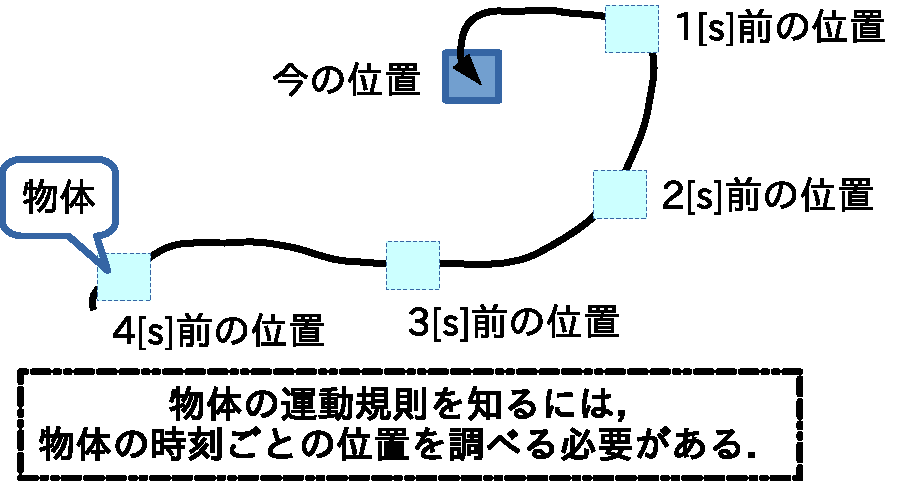
\includegraphics[keepaspectratio, width=7.2cm,height=3.72cm,clip]{henka0001.pdf}
                            \caption{軌跡$=$時刻ごとの位置の記録}
                            \label{fig:henka0001}
                        \end{center}
                    \end{figure}

%       %======================================================================
%       %  SubSection
%       %======================================================================
        \subsection{位置の時間変化の図示}
        物体の位置の時間変化を1つの図で表現する場合,
        次のように書ける.

        最初の位置を $\br_{1}$ として,次の位置 $\br_{2}$ に移動したという場面を考える.
        $\br_{1}$ から $\br_{2}$ に変化したのであるから,位置の変化分 $\br$ は
        \[
            \br = \br_{2} - \br_{1}
        \]
        とかける.
        \begin{figure}[hbt]
            \begin{center}
                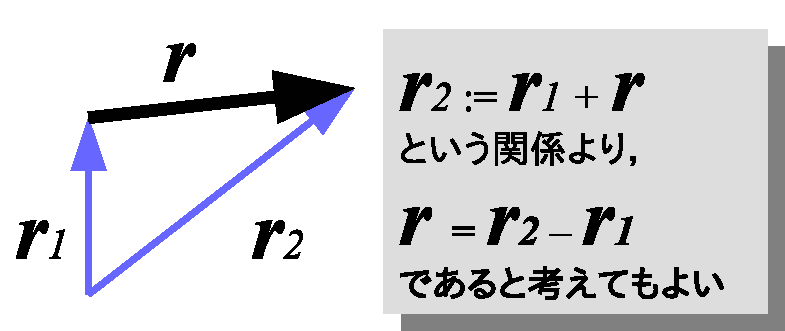
\includegraphics[keepaspectratio, width=6.2cm,height=3.2cm,clip]{ichi_henka.pdf}
                \caption{ベクトルの引き算}
                \label{fig:ichi_henka}
                \end{center}
        \end{figure}


%       %======================================================================
%       %  SubSection
%       %======================================================================
        \subsection{1次元(直線)上の速度}
                最初に,直線上を動く物体の様子について考えてみる.
                物体が直線上を運動するとき,物体は様々な速さで動くだろう.
                また,物体は直線上を右から左へ,もしくは左から右へ気まぐれに
                動くだろう.このような物体の運動を記述するにはどうすればよい
                だろうか.

                物体は直線上を動くと仮定しているので,物体は必ず直線上に存在し,$x(t)$ とい
                う1つの数で表現できる.
                物体が“動く”ということは, \textbf{時刻変化に伴って位置を変える} というこ
                とである.従って,
                時刻の変化 と 位置の変化 を考えれば物体の速さを表現できると考えられる.では,
                時刻の変化と位置の変化
                をどのように用いれば,速度を表現できるだろうか.その解決方法は,
                時刻の変化に対してどの程度の位置が変化するかという
                ことを表現すればよい.具体的に,2秒間で5[m]進む時の速さ と,
                3秒間で8[m]を進むときの速さ を考えてみよう.どちらが速いだろうか.
                これを考える場合,1秒間に対する移動距離を計算すればよい.
                2秒間で5[m]を進むのであれば,1秒間に2.5[m]進んでいて,
                3秒間で8[m]を進むのであれば,1秒間に2.6...$\cong$2.67[m]進んでいることになる.
                すなわち,3秒間で8[m]を進む方が速いと結論される.
                この具体的な計算で,距離を時間で割ることで1秒間に進む距離を計算し,
                その大きさによってどちらが速く動くかの結論を下した.
                これを一般の場合に拡張して,時間 $\Delta t$ の間に,物体
                の位置が $\Delta x$ だけ変化したとき,その速さは $\Delta x/\Delta t$ で
                表現されると言える.これ以降では速さを表現する記号として $v$ を用いることにする.
                すなわち,
                \begin{align}
                    v:=\frac{\Delta x}{\Delta t}
                \end{align}
                である.

                この式を見れば,同じ距離でも,より短い時間で
                その距離を変化するほうが速さが大きいと言える.
                また,同じ時間でもより大きな距離を
                移動したほうが早いともいえる.

                この速さの式をもう少し考察していこう.
                例えば,
                最初の状態で物体が位置 $x_{1}$ にあって,このときの時刻が $t_{1}$ であったとす
                る($x_{1}=x(t_{1})$).
                その後,物体が位置 $x_{2}$ へ動き,このときの時刻が $t_{2}$ であるとす
                る($x_{2}=x(t_{2})$).
                とすると,物体は時刻が $t_{1}$ から $t_{2}$ へ変化したとき,
                位置が $x_{1}$ から $x_{2}$ に変化したことになる.
                \begin{figure}[hbt]
                    \begin{center}
                        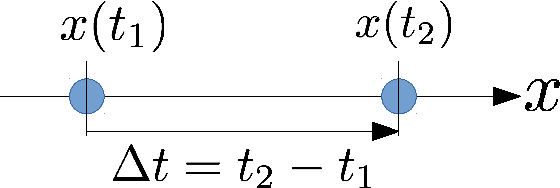
\includegraphics[keepaspectratio, width=6cm,height=3cm,clip]{sokudo1.pdf}
                    \end{center}
                    \label{fig:sokudo1}
                    \caption{速度1}
                \end{figure}

                $t_{1}$ と $t_{2}$ の時間間隔を $\Delta t$ と書いたとき,
                \begin{align}
                    \Delta t=t_{2}-t_{1}
                \end{align}
                と書ける.また同様に,
                位置も変化しているので,この位置の変化分は
                \begin{align}
                    \Delta x=x_{2}-x_{1}
                \end{align}
                と書ける.
                すると,物体の位置 $x_{1}$ から位置 $x_{2}$ へ向かうときの速さ $v$ は
                \begin{align}
                    v=\frac{\Delta x}{\Delta t}=\frac{x_{2}-x_{1}}{t_{2}-t_{1}}
                \end{align}
                となる.
                さらに,速さの式を次のように変形してみる.
                \begin{align}
                    \Delta x=v\Delta t
                \end{align}
                この式は,1次方程式の形をしている.変数は $\Delta t$ で
                あり,この変化に伴って $\Delta x$ も変化する.
                そして $v$ は変化の割合である.
                このように見れば,速さを図示して考えられる.
                1次方程式の変化の割合は,図で表現すれば,\textbf{傾き} として
                現れることになる.しかしこれには少々問題がある.
                これによって,速さ $v$ は
                わかるが,これは物体が位置 $x_{1}$ から位置 $x_{2}$ へ向かうときの
                平均的な速さでしかないのである.図\ref{fig:Sokudo2}を見てほしい.
                \begin{figure}[hbt]
                    \begin{center}
                        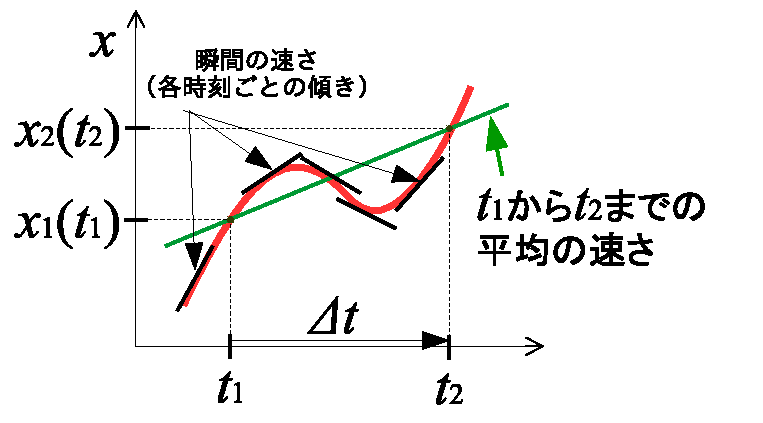
\includegraphics[keepaspectratio, width=7.2cm,height=3.88cm,clip]{Sokudo2.pdf}
                        \caption{速度2}
                        \label{fig:Sokudo2}
                    \end{center}
                \end{figure}

                実際の物体の速度は,各時刻で赤線の傾きであるのにもかかわらず,
                上の速さの式は,緑色の線の傾きというように
                みなされる.すなわち,
                位置 $x_{1}$ から位置 $x_{2}$ まで,
                速さが一定であるとみなされているのである.そのため,このままでは,
                ある特定の時刻における物体の速さが知りたいときには,
                速さの式は役に立たない.平均の速度だけしか考えることしか
                できないからである.

                そこで,次のように速さの式を
                いじってみる.例えば,時刻 $t_{1}$ を における
                物体の速度を知りたいとする.このとき,\textbf{時刻 $t_{2}$ を
                時刻 $t_{1}$ に近づけていけば,時刻 $t_{1}$ における
                物体の速度を得られる.}$\Delta t=t_{2}-t_{1}$ の関係式から,
                $t_{2}$ について解けば,
                \begin{align}
                    t_{2}=t_{1}+\Delta t
                \end{align}
                である.
                従って,時刻 $t_{2}$ を時刻 $t_{1}$ に近づけるとは,
                $\Delta t$ を0に近づけることと同じである.
                ところで,$\Delta t$ を0に近づけると,
                それに伴って位置も変化してしまう.位置の変化分は,
                $\Delta x=x_{2}-x_{1}$ であった.時刻を含めて
                詳しく書くと,
                \begin{align}
                    \Delta x=x(t_{2})-x(t_{1})
                \end{align}
                である.さらに,$t_{2}=t_{1}+\Delta t$ であるから,
                \begin{align}
                    \Delta x=x(t_{1}+\Delta t)-x(t_{1})
                \end{align}
                のように書ける.以上により,平均の速さの式は
                \begin{align}
                    v   &= \frac{\Delta x}{\Delta t}=\frac{x_{2}-x_{1}}{t_{2}-t_{1}}  \notag \\  \notag \\
                        &= \frac{x(t_{1}+\Delta t)-x_(t_{1})}{t_{1}+\Delta t-t_{1}} \notag \\  \notag \\
                        &= \frac{x(t_{1}+\Delta t)-x(t_{1})}{\Delta t}
                \end{align}
                のように変形できる.一般には,時刻 $t_{1}$ は任意の時刻で捉えることができるので,
                添え字の1をおとし,任意性を強調し,
                \begin{align}
                    v=\frac{x(t+\Delta t)-x(t)}{\Delta t}
                \end{align}
                と書ける.
                この式で,$\Delta t$ を0にもっていくのである.
                これを次のように表現する.
                \begin{align}
                    v=\lim_{\Delta t \to 0}\frac{x(t+\Delta t)-x(t)}{\Delta t}
                \end{align}
                この式の右辺を以下のように略記する.
                \begin{align}
                    \frac{\df x}{\df t}:=\lim_{\Delta t \to 0}\frac{x(t+\Delta t)-x(t)}{\Delta t}
                \end{align}
                この記号を用いて,速度は
                \begin{align}
                    v=\frac{\df x}{\df t}
                \end{align}
                のように表現する.但し注意することは,$\Delta t\not= 0$ を
                必ず満たしておくということである.

                図形的に考えると図\ref{fig:hayasa3}のようになる.
                \begin{figure}[hbt]
                    \begin{center}
                        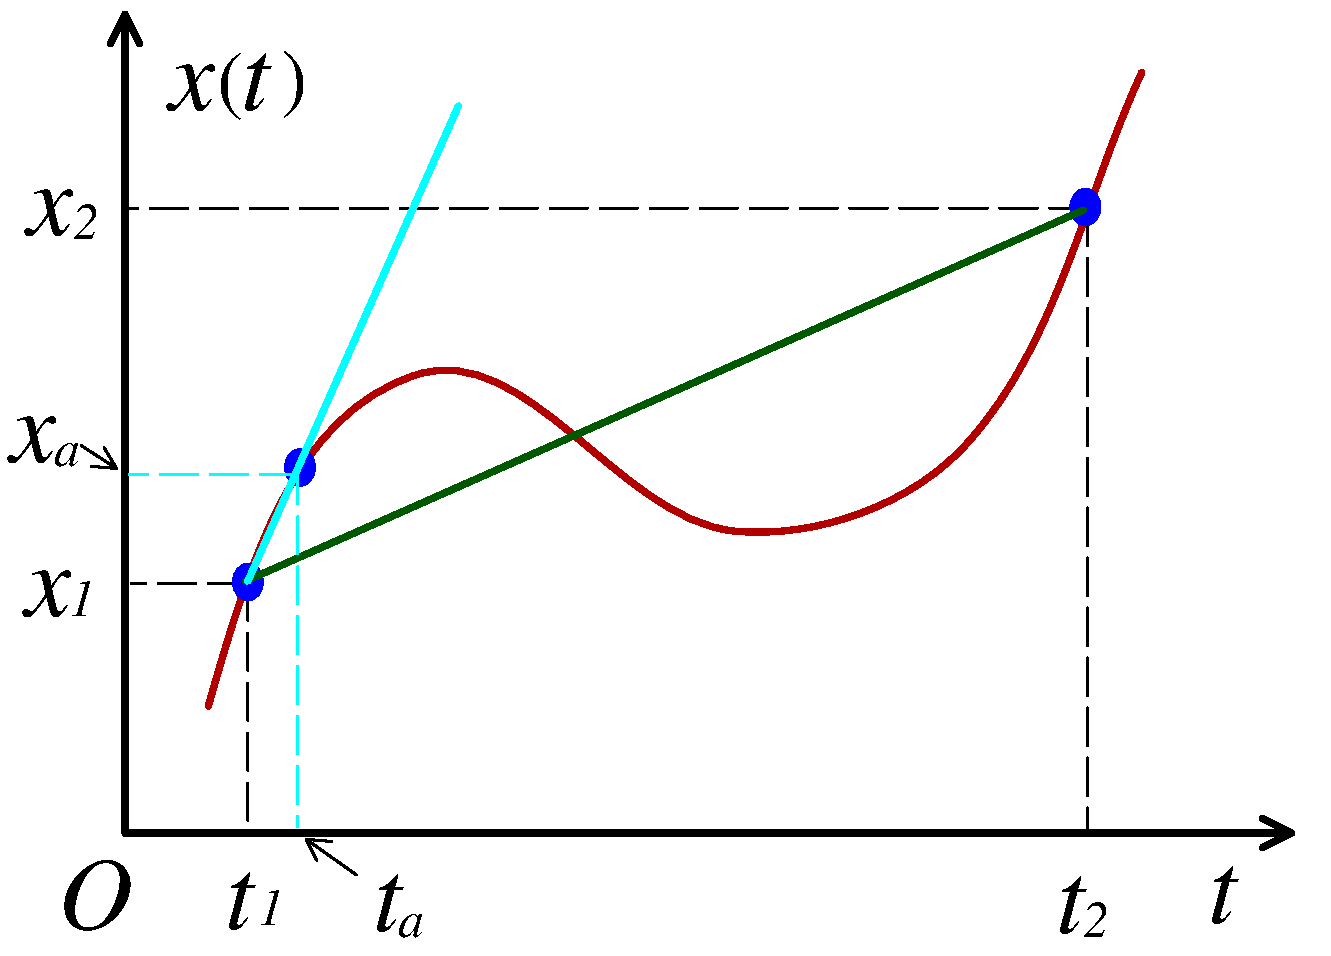
\includegraphics[keepaspectratio, width=7.2cm,height=5.73cm,clip]{hayasa3.pdf}
                        \caption{速度3}
                        \label{fig:hayasa3}
                    \end{center}
                \end{figure}

                このような図を“$x-t$ グラフ”という.
                時刻 $t_{2}$ を時刻 $t_{1}$ に
                近づけると,直線の傾き $v$ はある一定の値になる.この直線は
                水色の線で描いた.$t_{a}$ を $t_{1}$ へ
                近づいていくと,それに伴って $x_{a}$ も
                位置 $x_{1}$ へと近づいていく.但し,
                $x_{a}$ は $x_{1}$ に重ならないようにしなければならない.
                この直線が時刻 $t_{1}$ における
                瞬間の速さとなるのである.

                ここで注意しておく.それは,物体の位置と時刻の組 $(x(t),\,t)$ が
                2つ分かっていないと,速さはわからないということである.
                このことを考慮しないと,パラドクスを生んでしまうことになる.
                そのパラドクスとは,「飛ぶ矢のパラドクス」として有名である.
                次のようなものである.\\
                \begin{itembox}[l]{飛ぶ矢のパラドクス}
                動いている矢は,ある時刻を指定すれば,それに対応してある特定の
                位置で静止しているはずである.
                \end{itembox}\\

                簡単にいえば,ある時刻に撮った飛ぶ矢の写真を見ると,
                その矢は静止しているように見えるということである.
                しかし,2つの時刻で2つの位置の飛ぶ矢の写真をとれば,
                飛ぶ矢の平均の速度が求まる.もちろん,
                シャッターを押す速さが非常に速ければ,
                瞬間の速度を求められる
                \footnote{
                実際は
                そのようなことをせず,
                ビデオカメラを使うだろうが.}.

                さて,今までは速度の方向について何も考えてこなかったが,
                これは,正と負で表現できる.すなわち,左から右へ
                物体が移動するときに,物体は正方向に速度をもつ
                といい,逆に右から左に物体が移動するときには
                物体は負の向きに運動するという.


%       %======================================================================
%       %  SubSection
%       %======================================================================
        \subsection{2次元(平面)上の速度}
            2次元上,すなわち平面上における
            物体の位置は2つの方向で考える.この物体の位置は $\br=(x,\,y)$ のように
            表現される.    その速度についても2つの方向を考える必要がある.
            $x$ 方向の速度を $v_{x}$ また,$y$ 方向の速度 $v_{y}$ と
            したとき,$\bv=(v_{x},\,v_{y})$ である.
            これらはそれぞれ1次元における速度と同じように考えられて,
            \begin{align}
                v_{x}=\frac{\df x}{\df t}:=\lim_{\Delta t \to 0}\frac{x(t+\Delta t)-x(t)}{\Delta t} \notag \\
                v_{y}=\frac{\df y}{\df t}:=\lim_{\Delta t \to 0}\frac{y(t+\Delta t)-y(t)}{\Delta t}
            \end{align}
            である.

            ところで,位置が $\br=(x, y)$ と表せるので,
            速度は以下のようにも表せる.
            すなわち,
                \begin{align}
                    \bv=\left(v_{x} , v_{y}\right)
                       =\left(
                           \frac{\df x}{\df t},
                           \frac{\df y}{\df t}
                        \right)
                \end{align}
            である.


%       %======================================================================
%       %  SubSection
%       %======================================================================
        \subsection{3次元(空間)内の速度}
            3次元への拡張は容易だろう.3次元における物体の位置
            を $\br=(x,\,y,\,z)$ として,
            速度を $\bv=(v_{x}\,,\,v_{y}\,,v_{z})$ とすればよい.
            復習を兼ねてもう一度,形式的に速度について確認していく.

            時間が $t$ から $\Delta t$ だけ時間が経過したとき,
            位置は $\br(t)$ から $\br(t+\Delta t)$
            に変化する.すなわち,平均の速度 $\bar{\bv}$ は
                \begin{align}
                    \bar{\bv}
                    &= \frac{\br(t+\Delta t)-\br(t)}{t+\Delta t -t} \notag \\
                    &= \frac{\br(t+\Delta t)-\br(t)}{\Delta t }
                \end{align}
            である.知りたいのは「瞬間の速度」である.
            「瞬間の速度」を考えるために $\Delta t$ を0近づける.すると,
                \begin{align}
                    \bv
                    = \lim_{\Delta t \to \infty}\frac{\br(t+\Delta t)
                    -\br(t)}{\Delta t} \notag \\
                \end{align}
            となる.従って,
                \begin{align}
                    \bv=\frac{\df \br}{\df t}
                \end{align}
            である.これが \textbf{瞬間の速度} である.速度の単位は,[m/s] である.

            ところで,位置が $\br=(x, y, z)$ と表せるので,
            速度は以下のようにも表せる.
            すなわち,
                \begin{align}
                    \bv=\left(v_{x} , v_{y} , v_{z}\right)
                       =\left(
                           \frac{\df x}{\df t},
                           \frac{\df y}{\df t},
                           \frac{\df z}{\df t}
                        \right)
                \end{align}
            である.

            \begin{memo}{速度のを表す他の記号}
            速度は,$\df \bv/\df t$ と表現した.しかし,これを簡略化をして,以下のように書くことも
            あるので注意すべきだ.
                \begin{align}
                    \dot{\br} := \frac{\df \textit{\textbf{}v}}{\df t}.
                \end{align}
            \end{memo}

%       %======================================================================
%       %  SubSection
%       %======================================================================
        \subsection{速度の合成}
            今,人間 $A$ が速度 $\bv_{A}$ の等速で運動をしているとする.
            このとき,$A$ は 物体が速度 $\bv_{\mbox{物体}}$ をもって運動している のを見たとする.
            自分から見た物体の速度 $\textit{\textbf{V}}$ はどのようになるかを計算する.
            これは,ガリレイの \textbf{速度の合成則} によると,
                \begin{align}
                    \textit{\textbf{V}}=\bv_{\mbox{物体}}-\bv_{A}
                \end{align}
            の関係がある.この関係は,速度のベクトル和として考えられることによる.
            このように,$A$ から見た相手の速度 $\textit{\textbf{V}}$ のことを \textbf{相対速度} という.
            自分の速度を基準に, $\bv_{A}=0$ としたとき,
             $\textit{\textbf{V}}=\bv_{\mbox{物体}}$ となる.すなわち,
             自分は静止していて,動いているのは物体である主張できる.

            逆に,別の人 $B$ が物体の上から$A$を見るときを考える.$B$ は物体と共に運動している
            ことから,$\bv_{\mbox{物体}}=0$ とみなす.従って,動いているのは,$A$ であると主張できる.
            つまり,観測者によって 観測者自身の速度 が異なるので,物体の速度は 観測者によって 異なって見えるのである.
            (ここでは,観測者の立場によって,物体が動いていたり,止まっていたりしていた.)観測者の立場によって,
            互いの速度の主張は逆である.これが相対速度といわれる理由である.
            とすると,このままでは“絶対に正しい”とできる速度が存在しないことになる.
            従って,今まで,「速度」とか「加速度」とかという言葉を使ってきたが,何に対する 速度 または 加速度 であるのかを全く
            断っていなかった.この「何に対する」の『何』にあたるものが,速度や加速度の基準である.
            \begin{figure}[hbt]
                \begin{center}
                    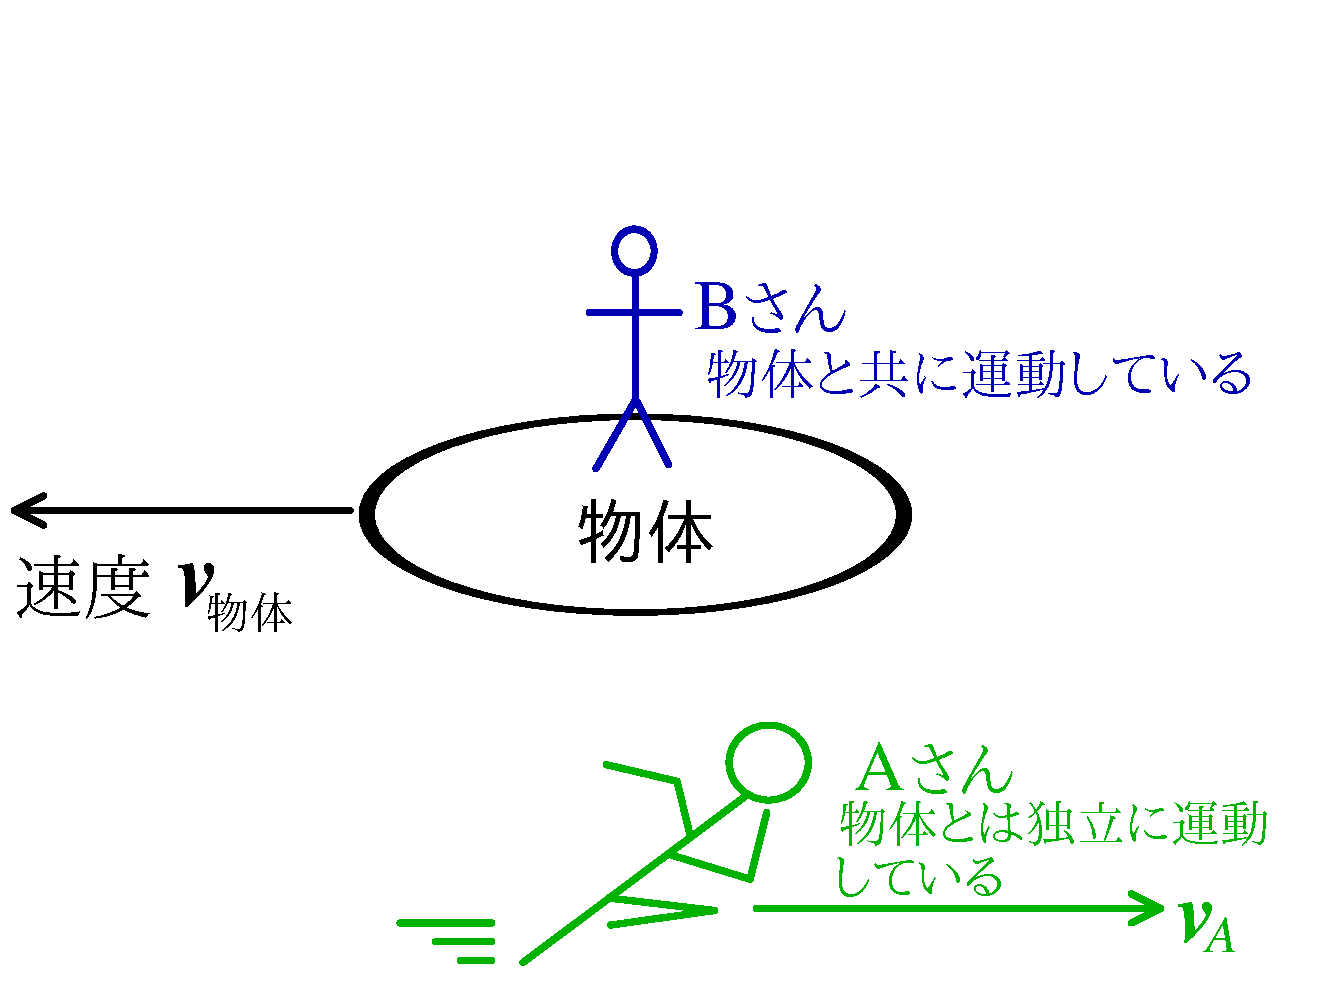
\includegraphics[keepaspectratio, width=7.2cm,height=5.92cm,clip]{soutaisokudo.pdf}
                    \caption{相対速度(Aから見た物体の速度 と Bから見た物体の速度)}
                    \label{fig:soutaisokudo}
                \end{center}
            \end{figure}

            \begin{memo}{数式と実際の現象}
                いよいよベクトルや微分,さらにはベクトルの微分と,数式が出てきは
                じめた.
                最初に戸惑うのは,数式と数式で表現されている現象との関係だろう.
                あたりまえのようだが,これについては問題を解くなりしていくしかない.
                物理学は実際の現象を数式で表す.逆にいえば物理における数式は何らかの
                物理現象を表現していると言える.式を見て,その式の内容を具体的な例で
                イメージできるように
                なるとよい.例えば,位置 $\br$ と表現されていたら,この具体的なイメ
                ージは,
                自分が原点に立っていて,その位置を指で示していることを考えればよい.
                速度 $\bv$ といわれたら,
                一定の速度で走る自転車を思い浮かべればよい.一定の速度で走るということは,
                常に時間変化 $\Delta t$ に対する自転車の変位 $\Delta\br$ が一定であることから,
                \begin{equation*}
                    \frac{\Delta \br}{\Delta t}=\mathrm{const(\mbox{一定})}=\bv
                \end{equation*}
                ということである.時間微分は,ある量(ここでは変位$\Delta \br$)時間変化に
                対する変化の割合を
                表現している.このように,式と現象が自身の中で,具体例を持って認識できる
                ようになるとよい.
            \end{memo}


%   %==========================================================================
%   %  Section
%   %==========================================================================
    \section{加速度の表現方法}
        \begin{mycomment}
            \textbf{加速度} とは,速度の時間変化具合を表す量である.
            速度を考えた時と同様に,加速度も1次元の場合から3次元の場合と,
            順を追って考えてくことにしよう.
        \end{mycomment}

%       %======================================================================
%       %  SubSection
%       %======================================================================
        \subsection{1次元(直線)上の加速度}
            一次元,つまり,直線的に運動する物体の速度 $v_{x}(t)$ は
            位置 $x(t)$ の時間変化 $\df / \df t$ として定義された.
            定義された.定義式は次の通りであった.
                \begin{align}
                    v_{x}(t) := \frac{\df x(t)}{\df t}
                              = \lim_{\Delta t \rightarrow 0}\frac{x(t+\Delta t)-x(t)}{\Delta t}.
                \end{align}

            ここでは更に,“速度の時間変化”を考える.この速度の時間変化を \textbf{加速度} と
            いう.以下に加速度を定義していこう.

            ある時刻 $t_{0}$ における物体の速度を $v_{x0}$ としたとき,
                \begin{equation*}
                    v_{x0} = v_{x}(t_{0})
                \end{equation*}
            という式が成り立つ.そして,次の時刻 $t_{1}$ における物体の速度 $v_{x1}$ は,
                \begin{equation*}
                    v_{x1} = v_{x}(t_{1})
                \end{equation*}
            と書ける.つまり,時刻 $t_{0}$ から $t_{1}$ までの間に,
            物体の速度は $v_{x0}$ から $v_{x1}$ に変化したことになる.
            時刻の変化(時間)を $\Delta t$,速度の変化を $\Delta v$ とし,
                \begin{align*}
                    \Delta t &= t_{1}  - t_{0}   \\
                    \Delta v &= v_{x1} - v_{x0}
                \end{align*}
            と置けば,加速度 $a_{x}$ は以下のように定義できる.すなわち,
                \begin{align}
                    a_{x} := \frac{\Delta v}{\Delta t}
                \end{align}
            である.これにより,加速度が速度の時間変化で定義されることが,
            示せた.

            もう少し,加速度の定義式を具体化していこう
                \footnote{
                    今まで置いた文字を展開していくことになる.効率の悪い説明だが,気にしない.
                }.
                \begin{align*}
                    a_{x} &= \frac{\Delta v}{\Delta t}                     \\
                          &= \frac{v_{x1} - v_{x0}}{\Delta t}              \\
                          &= \frac{v_{x}(t_{1}) - v_{x}(t_{0})}{\Delta t}  \\
                          &= \frac{v_{x}(t_{1}) - v_{x}(t_{0})}{\Delta t}  \\
                          &= \frac{v_{x}(t_{0}+\Delta  t) - v_{x}(t_{0})}{\Delta t}.
                \end{align*}
            ここで,$\Delta t = t_{1} - t_{0}$ から $t_{1} = t_{0}+\Delta  t$ を使った
                \footnote{
                    書くまでもないか$\cdots$.
                }.
            最後に,右辺に対して,$\Delta t \rightarrow 0$ の極限をとろう.
                \begin{align}
                    a_{x} = \lim_{\Delta t \rightarrow 0}
                            \frac{v_{x}(t_{0}+\Delta t) - v_{x}(t_{0})}{\Delta t}.
                \end{align}
            時間 $t$ による微分の記号 $\df/\df t$ を使うことで,速度が正確に定義できるようになった.
            すなわち,
                \begin{align}
                    a_{x}    :=\frac{\df v_{x}(t)}{\df t}
                              =\lim_{\Delta t \rightarrow 0}
                               \frac{v_{x}(t_{0}+\Delta t) - v_{x}(t_{0})}{\Delta t}.
                \end{align}

            更に一般化しよう.今までは,時刻 $t_{0}$ における物体の加速度を求めていたが,
            これを任意の $t$ で置き換えよう.
            そして,改めて,今度は正式に,加速度を次式で定義しよう.
                \begin{align}
                    a_{x}(t) :=\frac{\df v_{x}(t)}{\df t}
                              =\lim_{\Delta t \rightarrow 0}
                               \frac{v_{x}(t+\Delta t) - v_{x}(t)}{\Delta t}.
                \end{align}
            上式で,左辺の加速度の表現に,時刻 $t$ が独立変数であることを,
            明記するようにした.

            \begin{memo}{速度$\cdot$位置$\cdot$加速度の関係}
                速度 $v_{x}(t)$ が,$v_{x}(t) := \df x/ \df t$ と定義
                されるので,次の関係が成立している.
                \begin{align}
                    a_{x}(t) := \frac{\df v_{x}(t)}{\df t} := \frac{\df^{2} x(t)}{\df t^{2}}.
                \end{align}
                加速度の表現として,
                    \begin{equation*}
                        \frac{\df^{2} x(t)}{\df t^{2}}
                    \end{equation*}
                というものが,最もよく用いられる.

                「加速度は,位置に関する二階微分で定義される」という(見たまんまだ).
            \end{memo}

%       %======================================================================
%       %  SubSection
%       %======================================================================
        \subsection{2次元(平面)上の加速度}
            二次元の場合の加速度も,次元が増えただけで,考えることは一次元の
            場合と同じ.違いは,一次元の場合は1方向($x$ 軸)のみで考えればよ
            かったところを,二次元の場合は,2方向($x,\,y$)を考慮する点のみ.

            2つの方向を $x$ 軸,$y$ 軸とする.$x$ と $y$ 軸はそれぞれ独立だから,
            2つを別々に考えれば良い.どの方向を向いても,加速度の定義を変更する
            必要はない
                \footnote{
                    \textbf{空間の等方性} より.空間の方法性とは,
                    どの向きに運動しようが,その物体に対する
                    物理法則は不変である,という仮説のことを言う.
                }.
            つまり,1方向で考えたことが,そのまま残りの方向にも成立するということ
                \footnote{
                    してもらわないと困る.というか,成立するものとして,定義される.
                }.

            なので,上で考えた1次元の場合の式を,2方向に適用するだけで良い.
            次のように2方向の場合の加速度が定義できる.
                \begin{align}
                    \ba (t) := \frac{\df \bv(t)}{\df t}
                             = \left(
                                   \frac{\df^{2} x(t)}{\df t^{2}},\,\;
                                   \frac{\df^{2} y(t)}{\df t^{2}}
                               \right).
                \end{align}

            ただし,表記上の問題として,位置$\cdot$速度$\cdot$加速度
            をベクトル表記(太字)にした.

%       %======================================================================
%       %  SubSection
%       %======================================================================
        \subsection{3次元(空間)内の加速度}
            3次元になろうが,やることはこれまでと同じ.
            3次元空間内における加速度を $\textit{\textbf{a}}$ と表すと,
                \begin{align}
                    \textit{\textbf{a}} := \frac{\df \bv}{\df t}
                \end{align}
            である.考え方は速度のときと同じである.
            つまり,加速度とは速度の時間変化のことである.
            速度が時間の経過とともに速くなったり,逆に遅く
            なったりしたとき,
            その変化の具合が加速度である.

            また,速度の定義式から,以下のようにも加速度を表せる.
            すなわち,
                \begin{align}
                    \textit{\textbf{a}} &= \left( a_{x} , a_{y} , a_{z} \right) \notag \\
                    &= \left( \frac{\df v_{x}}{\df t} , \frac{\df v_{y}}{\df t} ,\frac{\df v_{z}}{\df t} \right)  \notag \\
                    &= \left( \frac{\df^{2}x}{\df t^{2}},  \frac{\df^{2}y}{\df t^{2}},  \frac{\df^{2}z}{\df t^{2}} \right) \notag \\
                    &= \frac{\df^{2}\br}{\df t^{2}}
                \end{align}
            とも表現できる.
            加速度が正の場合は,速度が上がっていくことを意味する.
            また,加速度が負の場合は,速度が下がっていくことを意味する.
            もちろん,加速度が 0 であれば,速度変化はないということである.

            加速度の単位は $[\rm{m/s^{2}}]$ である
                \footnote{
                    $[\rm{m/s^{2}}]$ はメートル毎秒毎秒とよむ.
                }.

            \begin{memo}{変化の記述}
                上に,「数式と物理現象は互いに関連していている」
                というようなことを書いた.そして,数式を見たときに,
                「それを現象を具体的な例で想像できることが大切である」
                とも書いた.しかし,具体的に式をイメージする方法を
                示していなかった.そこで,ここではこの例
                    \footnote{
                        当然,ここで紹介するのは,その単なる一例であり,これが全てではない.
                        むしろ,人ぞれぞれで,想像の仕方が異なっているはずである.
                        従って,想像できるようであれば,この節を読みとばしてかまわない
                        -----むしろ混乱するだろうから,読み飛ばすべきかも知れない.
                    }
                として,また,今までの復習を兼ねて,
                いまの私の考える微積分と物理現象を考えたい.


                物体は大きさをもっているが,この物体の運動を考えるときには物体の大き
                さを無視したほうが計算上都合がよい.
                物体の重心の運動を追うことで,物体の運動の軌跡を得ることができる.
                物体をこの重心部分にギュギュ!!と押しつぶして
                大きさをなくした点を考える.このような点のことを \textbf{質点} という.
                力学では,剛体の場合を除いて,物体の運動を考える
                ときは,質点の運動のことを考える.以下では,「物体」と書かれていたのなら,
                それは,特に断りのない限り,質点と同義であるとする.

                物体の運動を語るには,最初に,物体の \textbf{位置} を表現しなければならない.
                物体の位置は \textbf{座標} を用いて表現される.
                簡単のために,自身の居る点を原点 O にとろう.
                位置を表す記号として,$\br$ と表現する.つまり,物体の位置は
                \begin{equation*}
                \br =(\,x\,,\,\,y\,,\,\,z\,)
                \end{equation*}
                のように表現される
                \footnote{
                座標としては直交座標でないといけないという制約はないが,ここでは一番わか
                りやすいと思われる
                座標としてこの座標をとった.
                }.位置については,そのイメージをすることは容易だと思う.自分が原点にいて
                ,その点を指でさしている,というイメージ
                をすればよい.

                次に,物体の \textbf{速度} を考える.物体の速度とは,位置の時間変化を表す量である.
                まず,“変化”をどのように数式で表現すればよいかを考える.
                量の変化を表すには,その変化の前と後で二つの量の差を考える必要がある.量の変化は,
                \begin{equation*}
                [\mbox{量の変化分}] = [\mbox{変化後の量}] - [\mbox{変化前の量}]
                \end{equation*}
                と計算される.上の式をもう少し格好をつけて書くと,量の変化分を表すときには,
                その量を表す記号の前に $\Delta$ を
                つける.変化する量を,例えば $x$ としたとき,変化分は $\Delta x$ と表現する
                \footnote{
                $\Delta$ は,デルタ と読む.
                }
                .従って,変化前の量を $x_{\mbox{変化前}}$,
                変化後の量を $x_{\mbox{変化後}}$ と表現すれば,
                \begin{equation*}
                \Delta x = x_{\mbox{変化前}} - x_{\mbox{変化後}}
                \end{equation*}
                となる.

                また,「Aに対するB」を考えるとき,これは比で表現できて,
                \begin{equation*}
                \frac{B}{A}
                \end{equation*}
                と数式表現できる.例えば,二人の子どもに,3つのクッキーを配るとしよう.子ども一人
                に対して,
                クッキーはどれくらい与えられるかを考えれば,3/2 個であることは容易に計算される.
                この 3/2 は,
                \begin{equation*}
                    \frac{3[\mbox{個]}}{2[\mbox{人]}}
                \end{equation*}
                という意味である.式の意味は,「子ども二人に対して,クッキーが3つ」である.これは,
                子ども一人あたりのクッキーの個数でもある(3/2[個/人]).

                変化を考えるとき,基本となるのはこの引き算と割り算であり,
                後はこの組み合わせである.
                変化の基準となるものを分母にし,変化の対象となるものを分子におく.
                具体的に表現するならば,
                \begin{equation*}
                    \frac{\Delta A}{\Delta x} = \frac{A(x_{2})-A(x_{1})}{x_{2}-x_{1}}
                \end{equation*}
                のようである.$x$ の関数である $A(x)$ を考えるとき,$x$ の変化 $\Delta x$ に対
                する $A$ の変化 $\Delta A$ が
                上式で表現されている.現象の変化を表す一般的な形は,この式のようになる.


                やっと速度について考えられるが,
                速度の定義は,時間変化 $\Delta t$ の間にどの程度位置の変化 $\Delta x$ が起こるかを
                表現する.つまり,時間変化 $\Delta t$ に対する位置の変化 $\Delta x$ であるから,
                \begin{equation*}
                \frac{\Delta x}{\Delta t}
                \end{equation*}
                と表現される.
                この式は,次のように考えるとよい.まず,時間 $\Delta t$ を1秒で一定としてみよう.
                このとき,一秒で進む距離が大きければ大きいほど速度が速くなることをこの式は表現する.
                私達の経験上においても矛盾はないだろう.また,逆に,位置の変化 $\Delta x$ を1メー
                トルで一定にして
                考えてみよう.この場合,1メートルを進む時間が短ければ短いほど速度が速くなる.1メー
                トルを1秒で
                進みのと,1メートルを0.1秒で進むのでは,完全に後者の方が速い.

                実際の速度の変化は,直交座標でいうところの,$x$,$y$,$z$ の3方向で変化する.
                これは,位置が3方向であることから,当然のことである.従って,速度も3つの向きをもつ.
                つまり,
                速度もまたベクトルである.

                式で速度に意味をもたせる時には,それに対応した文字を割当てるとよい.そこで,速度
                を表現する記号として,$\bv$ を
                使うことにしよう.このノートでは,「定義する」という意味をこめて,$:=$ を使う.
                その使用方法は,例えば,記号Aに
                Bという意味をもたせたい時に,「AをBというように定義する」というとき,A$:=$Bのよ
                うに書く.今の速度の定義の場合,
                記号Aに対応するのが $\bv$ であり,意味Bに対応するのが $\Delta \br/\Delta t$ であるか
                ら,速度の定義は次のように
                書き表される.
                    \begin{align}\label{sokudonosiki_1}
                        \bv := \frac{\Delta \br}{\Delta t}.
                    \end{align}

                しかし上の式では,前の項目で定義した速度の定義と記号が異なる.
                小さい変化という意味をこめて,$\Delta$ を使っている点である.
                この記号 $\Delta$ は有限の個数の範囲でたくさん分割したときの,その1つの区間という
                イメージで使用される.
                しかし,これはあくまでも近似的な考えである.理想的には分割個数を無限大にし,分割さ
                れた区間を無限小にしたい.
                そこで,微積分という手段を使う.
                微積分を用いることで,無限小の変化を扱うことができる.有限分割から無限分割にしたの
                で,当然,
                用いる記号も
                変えないといけない.すなわち,$\Delta$ を $\df$ に変えるということである.
                    \begin{align}\label{sokudonosiki_2}
                        \bv := \frac{\df \br}{\df t}.
                    \end{align}
                式(\ref{sokudonosiki_1})と式(\ref{sokudonosiki_2})の違いは,位置の変化を有限分割に
                して表すか,
                無限分割にして表すかの違いである.速度の定義は,無限分割の概念で定義するほうが適当
                であるから,
                式(\ref{sokudonosiki_2})が正式な速度の定義になる.

                上記はベクトルで書かれているが,これは,単なる以下の式の省略である.
                        \begin{align}
                            \left(
                                v_{x} ,\,
                                v_{y} ,\,
                                v_{z}
                            \right)
                            = \left(
                                \frac{\df {r}_{x}}{\df t} ,\,
                                \frac{\df {r}_{y}}{\df t} ,\,
                                \frac{\df {r}_{z}}{\df t}
                              \right)
                        \end{align}
            \end{memo}


    \section{躍度(加加速度,jerk)}\label{seq:jerk_define}
        理論構築には直接的に関係がないためか,力学の教科書では見かけないけど,
        加加速度(jerk)についても書いておこう.
        現実的には,加速度も時間変化する.この加速度の時間変化を \textbf{加加速度} という.
        \textbf{躍度} ともいう.個人的には,躍度という方を好む
            \footnote{
                加加速度だといい間違えたと思われて誤解されそうなので.
            }.
        英語だとjerk(ジャーク).躍度は,工学的な匂いが強い.

        一応式も書いておこう.加速度がベクトルであるから,躍度もベクトルになる.
        躍度を現す記号を$\bj$としよう
            \footnote{
                jerkからとったjである.後に使う仕事の記号jとは無関係.電気数学の虚数単位とも無関係.
            }.
        定義式は以下.
            \begin{align}\label{eq:jerk_define}
                \bj &:= \frac{\df \ba}{\df t} \\
                    &=  \frac{\df }{\df t} \left(\frac{\df \bv}{\df t}\right) \notag \\
                    &=  \frac{{\df}^{2} \bv}{{\df t}^{2}} \notag \\
                    &=  \frac{{\df}^{2} }{{\df t}^{2}} \left( \frac{\df \bx}{\df t} \right) \notag \\
                    &=  \frac{{\df}^{3} \bx}{{\df t}^{3}}. \notag
            \end{align}



